\documentclass[12pt,A4,A4pt]{article}

\usepackage{amsmath}
\renewcommand*\familydefault{\sfdefault} 
\usepackage[scaled]{helvet}
\renewcommand\familydefault{\sfdefault} 
\usepackage[T1]{fontenc}
%\usepackage[T1]{fontenc}
%\usepackage{arial} 
%\pagestyle{myheadings}{}
 %\markboth{left head}{right head}
\usepackage{amssymb}
%\usepackage{epsfig}
\usepackage{fancyhdr}
\usepackage{float}
%\usepackage[authoryear,round]{natbib}
\usepackage{apacite}
%\usepackage[sort&compress]{natbib}
\usepackage[pdftex]{graphicx}
\usepackage{color}
\usepackage[brazil]{babel}
\usepackage[utf8]{inputenc}
\usepackage{amsfonts}
\usepackage{textcomp}
\usepackage{tabularx}
\usepackage{multirow}
\usepackage{times}
\usepackage{multicol}
\usepackage{lscape}
\usepackage{subfig}
\usepackage{epstopdf}
\usepackage{setspace}
\usepackage{fancyhdr}
\usepackage{epigraph}
\usepackage{scrextend}
\usepackage[shortlabels]{enumitem}
\usepackage{ragged2e}


%\let\OLDthebibliography\thebibliography
%\renewcommand\thebibliography[1]{\OLDthebibliography{#1} \setlength{\parskip}{0pt}\setlength{\itemsep}{0pt plus 0.3ex}}

%\renewcommand{\chaptermark}[1]{\markboth{\MakeUppercase{#1}}{}}
%\renewcommand{\sectionmark}[1]{\markright{\MakeUppercase{#1}}{}}
\pagestyle{fancy}
\fancyhf{}
\renewcommand{\headrulewidth}{0cm}
%\renewcommand{\footrulewidth}{0}
\usepackage{pdfpages}
\usepackage{stackrel}
\usepackage[left=3cm, right=3cm, top=2.5cm, bottom=2.5cm]{geometry}
\newtheorem{exemplo}{Exemplo}
\newtheorem{definicao}{Definição}
\newtheorem{teorema}{Teorema}
\cfoot{{\fontsize{10pt}{\baselineskip}\selectfont \textbf{8\textsuperscript{o} MCSul / VIII SEMENGO - Universidade Federal do Rio Grande}}}



%%%%%
%tira os numeros da frente do autor
\makeatletter 
\renewcommand\@biblabel[1]{}
\makeatother
%%


\begin{document}
\pretolerance10000


\begin{figure}
\centering
\vspace{-1cm}
\begin{minipage}[c]{\textwidth}
\centering
    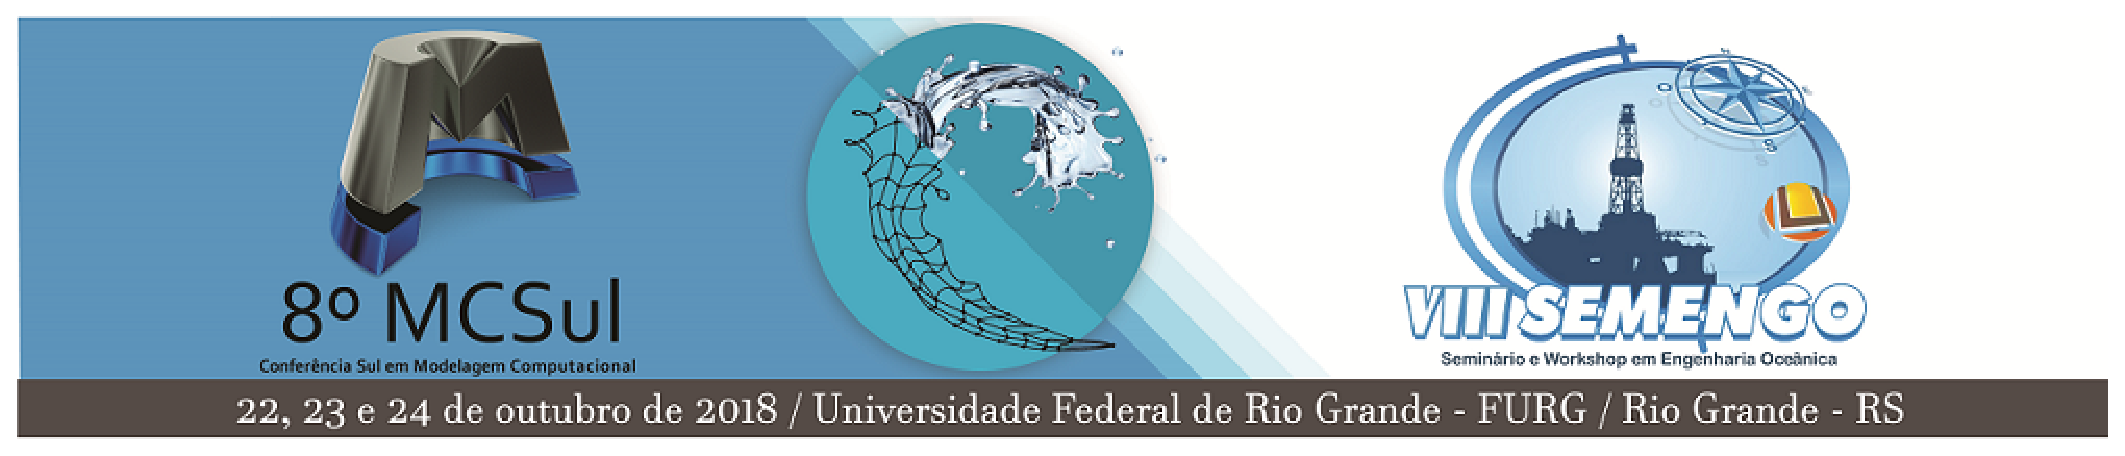
\includegraphics[width=6.2in]{cabecalho.eps}
\end{minipage}
\end{figure}



\begin{center}
\fontsize{16pt}{\baselineskip}\selectfont 
\textbf{{ANÁLISE DO ALGORITMO DE EVOLUÇÃO DIFERENCIAL APLICADO AO DESIGN CONSTRUCTAL DE UMA CAVIDADE EM FORMA DE DUPLO-T}}
\end{center}
\vspace{-0.9cm}
% \begin{center}
% \vspace{0.5cm}
% \textbf{\large{\textit{TÍTULO DO TRABALHO EM INGLÊS}}}
% \end{center}

\begin{flushright}
Gill V. Gonzales\footnote{Mestre, Instituto Federal Sul-Rio-Grandense - Campus Santana do Livramento, RS, Brazil, gillgonzales@ifsul.edu.br.}$^{,2}$

Liércio A. Isold\footnote{Doutor, Universidade Federal do Rio Grande - PPG em Modelagem Computacional, Rio Grande, RS, Brazil, liercioisoldi@furg.br.}

Luiz A. Oliveira Rocha\footnote{Doutor, Universidade do Vale do Rio dos Sinos - PPG em Engenharia Mecânica – São Leopoldo, RS, Brasil luizor@unisinos.br.}

Elizaldo D. dos Santo\footnote{Doutor, Universidade Federal do Rio Grande - PPG em Modelagem Computacional, Rio Grande, RS, Brazil, elizaldosantos@furg.br.}

Antônio J. Silva Neto\footnote{Doutor, Universidade do Estado do Rio de Janeiro, Instituto Politécnico, Nova Friburgo, RJ, Brazil, ajsneto@iprj.uerj.br.}

\end{flushright}

\begin{flushleft}
{\small \setstretch{0.5} \justify
\textbf{Resumo:} Neste trabalho é investigado o desempenho do algoritmo de Evolução Diferencial aplicado à otimização geométrica de um problema de transferência de calor. O problema consiste em uma cavidade em forma de Duplo-T inserida em um sólido com geração de calor constante e uniforme. As laterias do sólido estão em condições adiabáticas e o calor gerado só pode ser removido pela cavidade, a qual é mantida a uma temperatura prescrita. Portanto, a geometria da cavidade influência diretamente a performance térmica do problema. A definição dos graus de liberdade e restrições do problema é realizada através do método de Constructal Design. A otimização geométrica é realizada através do algoritmo de Evolução Diferencial. Neste estudo, são avaliados os parâmetros do algoritmo, tais como o operador de mutação, taxa de cruzamento, fator de amplificação do cálculo diferencial e número de iterações ou avaliação da função objetivo. O número de iteração está relacionado aos parâmetros que configuram o número de gerações e quantidade de indivíduos na população.  O objetivo principal do trabalho é avaliar os parâmetros do algoritmo de Evolução Diferencial e qual a influência na correta reprodução dos efeitos dos graus de liberdade estudados sobre a geometria ótima e performance térmica do problema. Os resultados indicam como mais adequadas as configuração dos parâmetros de taxa de cruzamento e fator de amplificação respectivamente com os seguintes valores 0,7 e 1,5. Estes parâmetros, em conjunto com operador de mutação identificado como de/rand/1/bin, tornaram os resultados do algoritmo mais robustos e necessitando de um menor número de avaliações da função objetivo para a obtenção das geometrias ótimas. A principal contribuição do trabalho é a recomendação de um conjunto de parâmetros adequados que adaptem o algoritmo de Evolução Diferencial ao problema estudado, tornando o algoritmo mais efetivo e robusto para a otimização geométrica do problema estudado.
%contagem de palavras: 298/300

\vspace{0.3cm}

\noindent\textbf{Palavras-chave:} Otimização Geométrica. Transferência de Calor. Constructal Design. Evolução Diferencial.}
\end{flushleft}


% \noindent\textbf{Abstract:} O resumo em inglês apresenta-se logo após o resumo em português. Sugere-se encaminhar o texto para ser traduzido por um profissional. Caso o artigo esteja em inglês, deve haver uma versão do título, resumo e palavras-chave em português ou espanhol.
% \vspace{0.3cm}

% \noindent\textbf{Keywords:} Keywords. Keywords. Keywords. Keywords. Keywords.}

\newpage
 \onehalfspacing
\section{Introdução}

 {\fontsize{12pt}{\baselineskip}\selectfont}
 
\hspace{0.5cm}A pesquisa em cavidades resfriadoras têm início no trabalho de \citeA{Biserni2004}, onde são propostas as formas elementares C e T. Neste trabalho \cite{Biserni2004}, o método de Constructal Design é aplicado para a definição do problema de otimização, assim como a avaliação da influência da geometria sobre a minimização da resistência térmica entre a cavidade e o sólido. O método Constructal Desing é baseado na Teoria Constructal (Bejan 1996), a qual defende que um princípio físico, a Lei Constructal, determina as formas e estruturas presentes na natureza, sendo a geometria o resultado da otimização da passagem de um fluxo em um sistema de escoamento. A Lei Constructal afirma que "Para um sistema de escoamento, animado ou inanimado, evoluir no tempo (sobreviver) é preciso que sua forma e estrutura também evoluam de forma a facilitar a passagem do fluxo",(Bejan e Lorente, 2011). Portanto, a geometria é o resultado de um processo de otimização da passagem do escoamento. É importante salientar que o método de Constructal Design (CD) não é o método de otimização. O CD determina os graus de liberdade, restrições e espaço de busca do problema para a avaliação da geometria. Para a otimização geométrica são aplicados métodos de otimização como a Busca Exaustiva ou métodos heurísticas como o Recozimento Simulado e Algoritmos Genéticos (Gonzales et al., 2015;Lorenzini et al., 2014)

Biserni (2004) concluiu que a cavidade em forma de T é mais eficiente que a primeira forma elementar em C, pois consegue adentrar melhor no domínio computacional investigado. A partir desta observação, formas mais complexas são investigadas, como se pode observar nos trabalhos de Lorenzine, Xie, assim como cavidades múltiplas. Por exemplo, no trabalho de Lorenzine et al. (2011) a cavidade proposta em foram de Y, foi até 66\% mais eficiente que a forma elementar T. Portanto, na literatura recente, é possível constatar que formas mais complexas possuem um maior desempenho na minimização da resistência térmica entre o sólido e a cavidade, para o mesmo tipo de problema e mantendo as mesmas restrições. Entretanto, quanto maior a complexidade da cavidade maior é esforço computacional necessário no processo de otimização geométrica, principalmente quando o método de otimização empregado é o método de Busca Exaustiva (BE), quando todas as possibilidades são simuladas. Neste sentido, com a proposta de minimização do esforço computacional e possibilidade de investigar outras características do problema, métodos heurísticos são utilizados no processo de otimização (Lorenzini et al., 2014;Gonzales et al., 2015; Biserni et al. 2017).


\section{Modelagem Matemática e Numérica}
\label{modelo}
\hspace{0.5cm}O modelo matemático...

\section{Otimização Geométrica}
\label{opt}
\hspace{0.5cm}A otimização geométrica...

\subsection{Constructal Design}
\label{ed}
\hspace{0.5cm}A otimização geométrica...


\subsection{Evolução Diferencial}
\label{ed}
\hspace{0.5cm}A otimização geométrica...

\section{Resultados}
\label{opt}
\hspace{0.5cm}A otimização geométrica...

\section{Conclusão}
\label{opt}
\hspace{0.5cm}A otimização geométrica...

%**********************************************************************************
\section*{Agradecimentos}
\hspace{0.5cm}Agradecimentos e outras seções não numeradas são criadas pela utilização de um asterisco posterior ao comando, \verb|\section*{Agradecimentos}|.

OBS: Parte dos textos utilizados neste modelo para exemplificar seções, quadros, tabelas, etc., foram gentilmente cedidos pela Revista Mundi\footnote{http://periodicos.ifpr.edu.br}, do IFPR.

%**********************************************************************************

\bibliographystyle{apacite}
\bibliography{referencial}


\end{document}
